\documentclass[12pt]{article}
\usepackage{amsmath, amssymb, geometry, graphicx, hyperref, setspace, float, subcaption}

% Page settings
\geometry{a4paper, margin=1in}
\setlength{\parindent}{0pt}
\setlength{\parskip}{1em}
\onehalfspacing

% Title and author
\title{Assignment 1: Experiments and Analysis}
\author{Isaak Wiebe, V01004501}
\date{\today}

\begin{document}

% Title Page
\maketitle
\tableofcontents
\newpage

% Section 1: Introduction
\section{Introduction}
A binary classification task was performed on the Spambase dataset to distinguish between spam and non-spam emails using various statistical learning models. The models were implemented using SciKit-Learn and NumPy, and visualizations were generated using Matplotlib. The goal of this analysis was to evaluate the performance of different machine learning techniques, including decision trees, random forests, and boosted decision stumps, in classifying emails. The dataset, sourced from the UCI Machine Learning Repository, contains features derived from email content, such as word frequencies and special characters, making it suitable for binary classification tasks.

---

% Section 2: Results and Analysis
\section{Part I: Separate Analysis}
This section details the individual performance of each model and the approaches taken to optimize their performance on the dataset. For each model, multiple configurations and pruning techniques were explored to identify the best fit for the data.

\subsection{Decision Trees}
Decision trees were implemented using four different pruning techniques to evaluate their impact on model performance and complexity:
\begin{itemize}
    \item \textbf{No pruning}: A fully grown tree without any constraints, which often leads to overfitting.
    \item \textbf{Minimum Cost-Complexity Pruning}: A method that balances tree complexity and accuracy by introducing a penalty for additional nodes.
    \item \textbf{Reduced Error Pruning (Gini Index)}: Pruning based on the Gini impurity measure, which minimizes misclassification.
    \item \textbf{Reduced Error Pruning (Just Error)}: Pruning based solely on classification error.
\end{itemize}

Figure \ref{fig:comparison} illustrates the resulting decision trees for each pruning method. The pruned trees are significantly smaller and less complex than the unpruned tree, demonstrating the effectiveness of pruning in reducing overfitting.

\begin{figure}[htbp]
    \centering
    % First row of graphs (2 graphs side by side)
    \begin{subfigure}{0.45\textwidth}
        \centering
        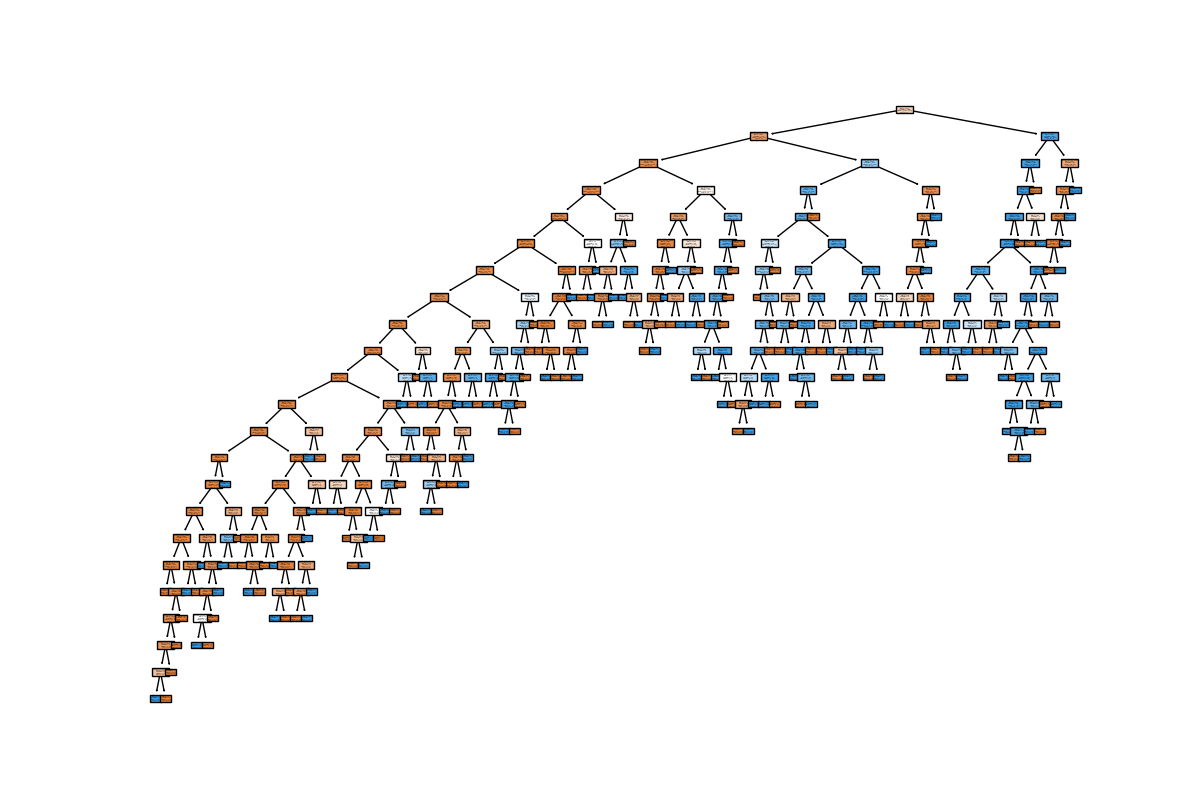
\includegraphics[width=\linewidth]{figures/Reduced Error Pruning/raw_tree.png}
        \caption{Raw Tree}
        \label{fig:method1}
    \end{subfigure}
    \hfill
    \begin{subfigure}{0.45\textwidth}
        \centering
        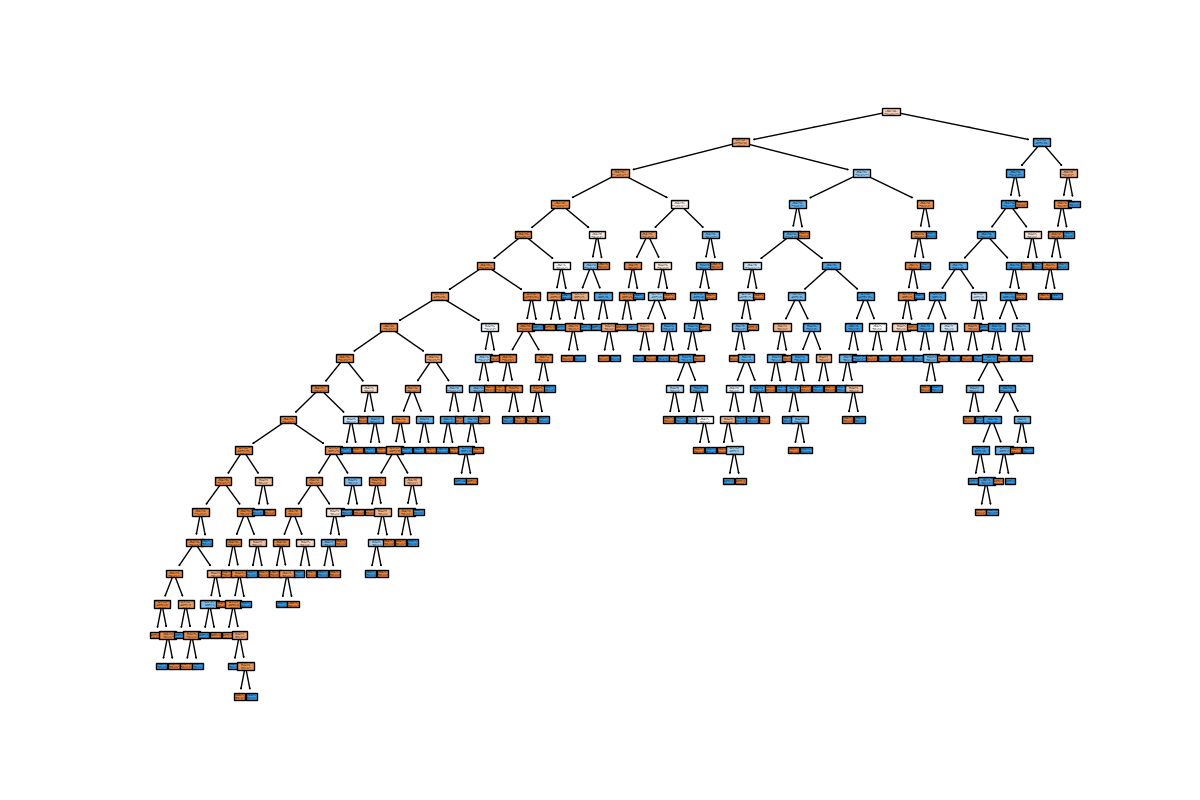
\includegraphics[width=\linewidth]{figures/Reduced Error Pruning/ccp tree.png}
        \caption{Cost-Complexity Pruning Tree}
        \label{fig:method2}
    \end{subfigure}
    
    % Second row of graphs (2 graphs side by side)
    \vskip\baselineskip  % Adds a line break between rows
    \begin{subfigure}{0.45\textwidth}
        \centering
        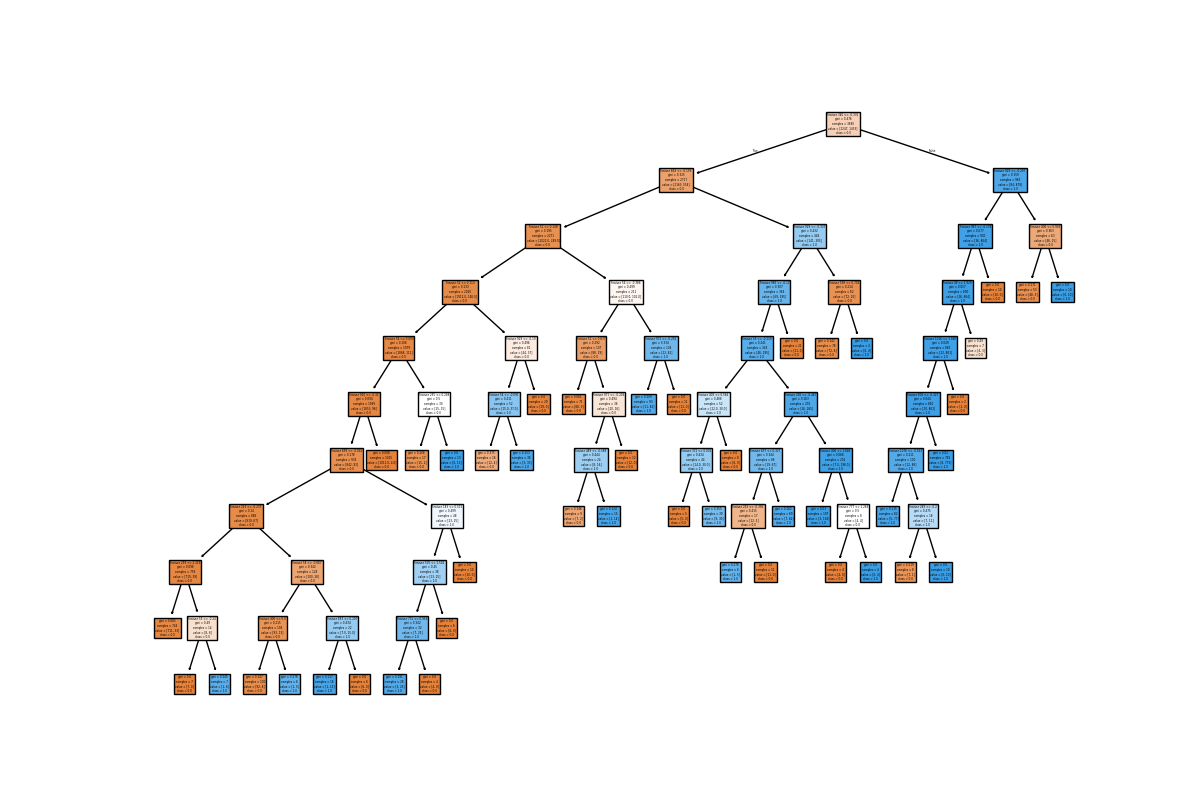
\includegraphics[width=\linewidth]{figures/Reduced Error Pruning/error_tree.png}
        \caption{Reduced Error Tree}
        \label{fig:method3}
    \end{subfigure}
    \hfill
    \begin{subfigure}{0.45\textwidth}
        \centering
        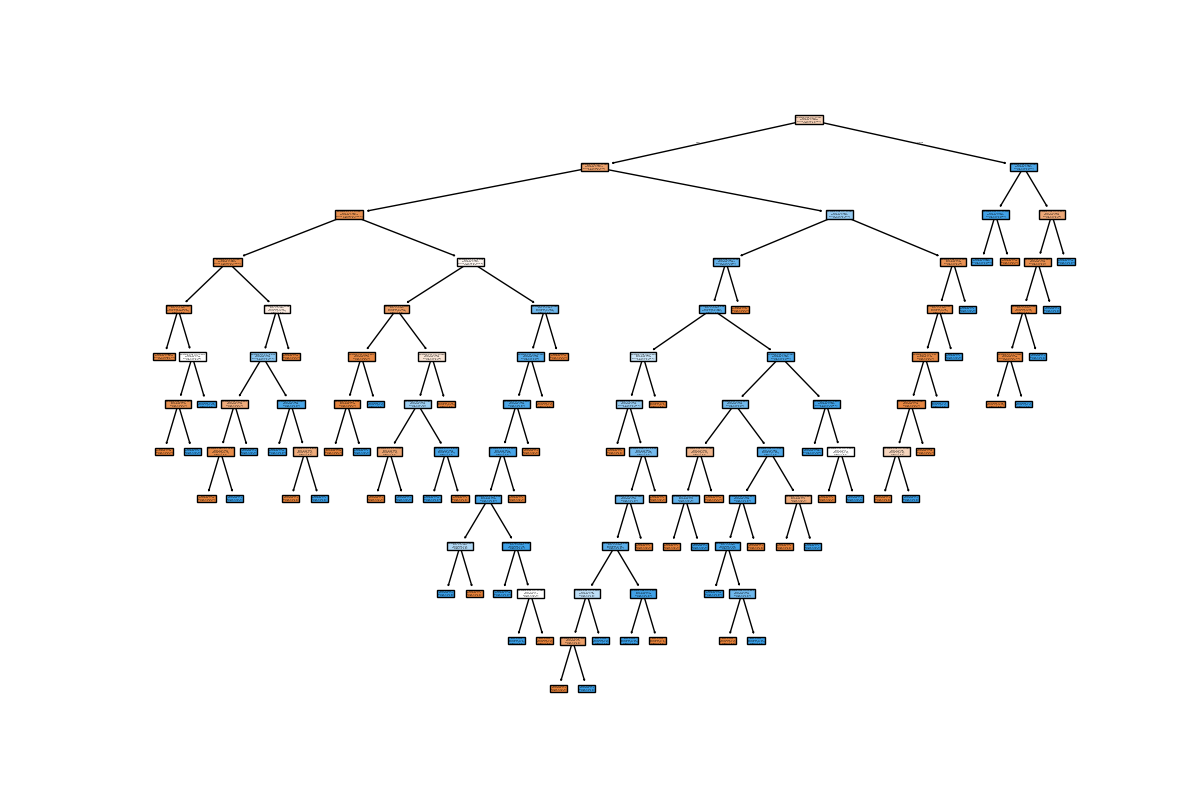
\includegraphics[width=\linewidth]{figures/Reduced Error Pruning/gini tree.png}
        \caption{Gini Index Tree}
        \label{fig:method4}
    \end{subfigure}

    \caption{Comparison of Decision Trees with Different Pruning Methods}
    \label{fig:comparison}
\end{figure}

To determine the optimal pruning parameters, the relationship between the pruning parameter (alpha) and model accuracy was analyzed. Figures \ref{fig:mcc}, \ref{fig:gini}, and \ref{fig:error} show these relationships for each pruning method.

\subsubsection{Minimum Cost-Complexity Pruning}
Figure \ref{fig:mcc} shows the trade-off between alpha and accuracy for minimum cost-complexity pruning. As alpha increases, the tree becomes simpler, but accuracy may decrease if pruning is too aggressive.

\begin{figure}[h!]
    \centering
    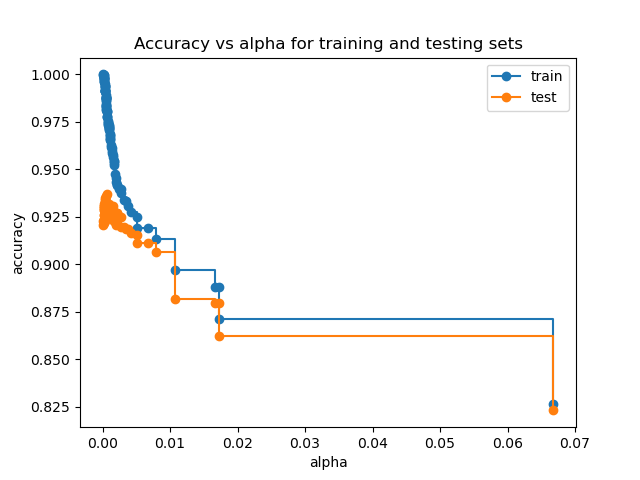
\includegraphics[width=0.8\linewidth]{figures/CCP/Accuracy vs alpha for train and test sets.png}
    \caption{Alpha vs. Accuracy for Minimum Cost-Complexity Pruning}
    \label{fig:mcc}
\end{figure}

\subsubsection{Reduced Error Pruning (Gini Index)}
Figure \ref{fig:gini} illustrates the relationship between alpha and accuracy for reduced error pruning using the Gini index. The Gini index measures the likelihood of misclassification, and pruning based on this metric helps balance accuracy and complexity.

\begin{figure}[h!]
    \centering
    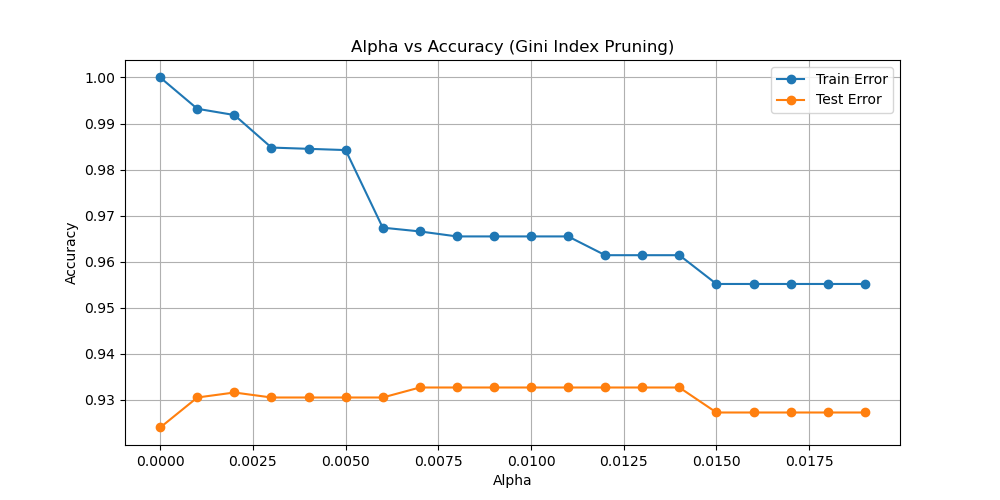
\includegraphics[width=0.8\linewidth]{figures/Reduced Error Pruning/gini alpha vs accuracy.png}
    \caption{Alpha vs. Accuracy for Reduced Error Pruning (Gini Index)}
    \label{fig:gini}
\end{figure}

\subsubsection{Reduced Error Pruning (Just Error)}
Figure \ref{fig:error} shows the relationship between alpha and accuracy for reduced error pruning based solely on classification error. This method is simpler but may not always yield the best balance between accuracy and complexity.

\begin{figure}[h!]
    \centering
    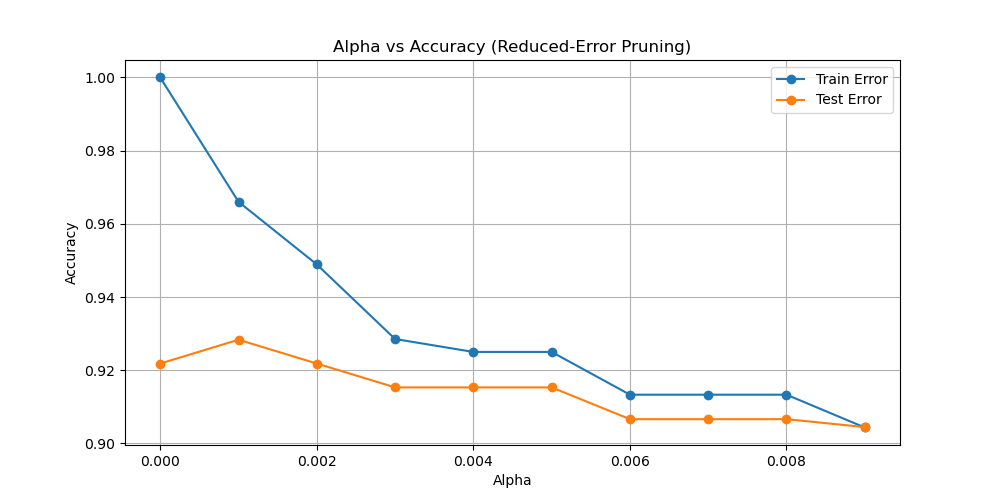
\includegraphics[width=0.8\linewidth]{figures/Reduced Error Pruning/alpha vs accuracy.png}
    \caption{Alpha vs. Accuracy for Reduced Error Pruning (Just Error)}
    \label{fig:error}
\end{figure}

\subsection{Random Forests}
Random forests were analyzed by varying ensemble size (number of trees) and maximum tree depth. The importance of each feature in the dataset was also evaluated, as shown in Figure \ref{fig:uh}. Figures \ref{fig:idk} and \ref{fig:smth} display the max depth, number of trees, and the corresponding error rates, respectively.

\begin{figure}[h!]
    \centering
    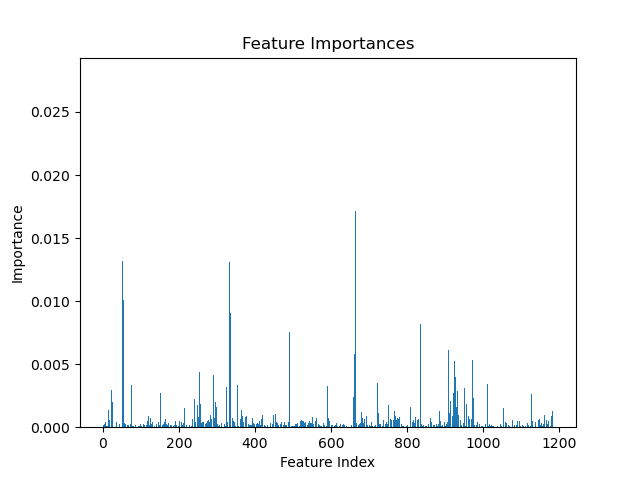
\includegraphics[width=0.8\linewidth]{figures/Random Forests/Feature Importance.png}
    \caption{Importance of Each Feature}
    \label{fig:uh}
\end{figure}

\begin{figure}[h!]
    \centering
    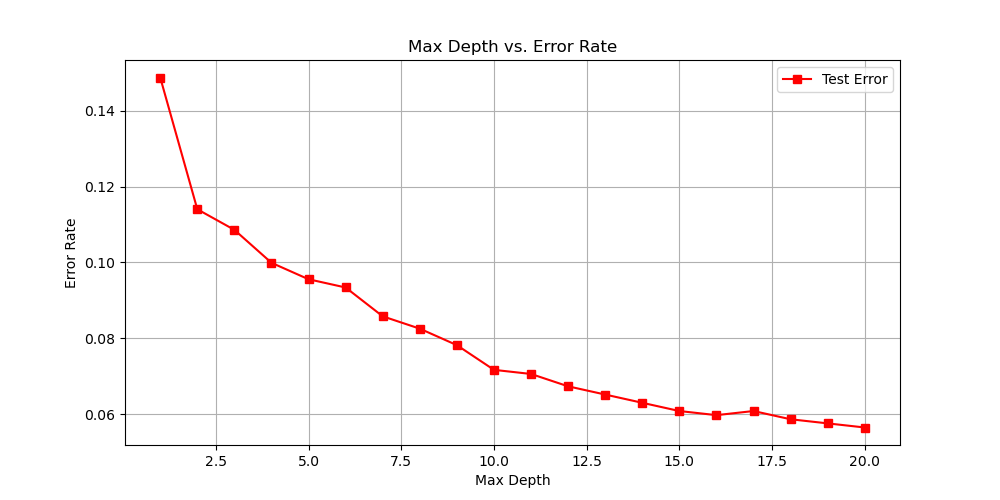
\includegraphics[width=0.8\linewidth]{figures/Random Forests/Max depth vs error rate.png}
    \caption{Max depth vs training and test error rate}
    \label{fig:idk}
\end{figure}

\begin{figure}[h!]
    \centering
    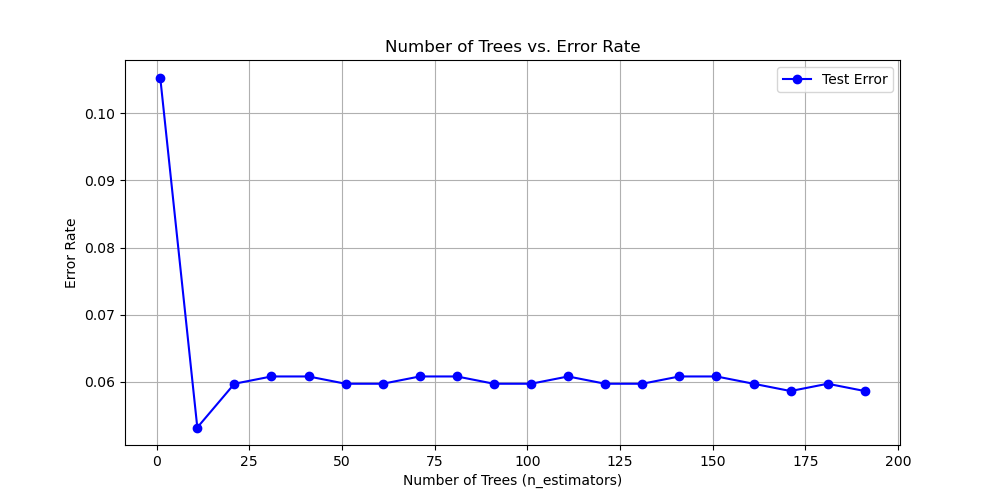
\includegraphics[width=0.8\linewidth]{figures/Random Forests/Number of trees vs error rate.png}
    \caption{Number of trees vs training and test error rate}
    \label{fig:smth}
\end{figure}

\subsection{Boosted Decision Trees}
AdaBoost, a boosting algorithm, was used to analyze boosted decision stumps. The ensemble size and stump weights were varied to evaluate their impact on error rates. This method combines multiple weak learners to create a strong classifier, often achieving higher accuracy than individual decision trees. The optimization methods are shown in figures \ref{fig:ada}, \ref{fig:boo} and \ref{fig:st}.

\begin{figure}[h!]
    \centering
    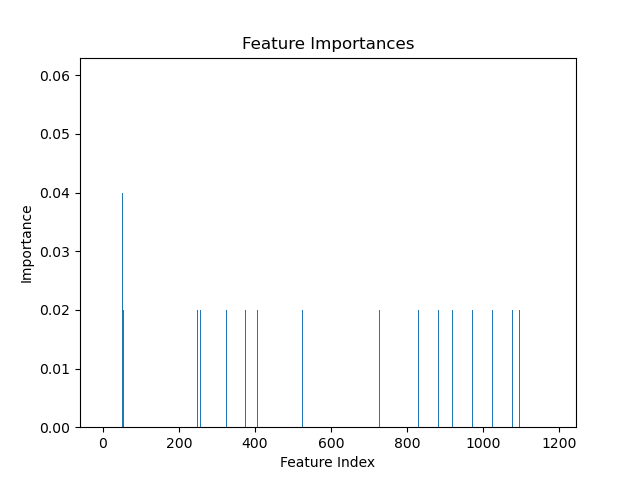
\includegraphics[width=0.8\linewidth]{figures/Boosted Trees/Feature Importance.png}
    \caption{AdaBoost Feature Importance}
    \label{fig:ada}
\end{figure}

\begin{figure}[h!]
    \centering
    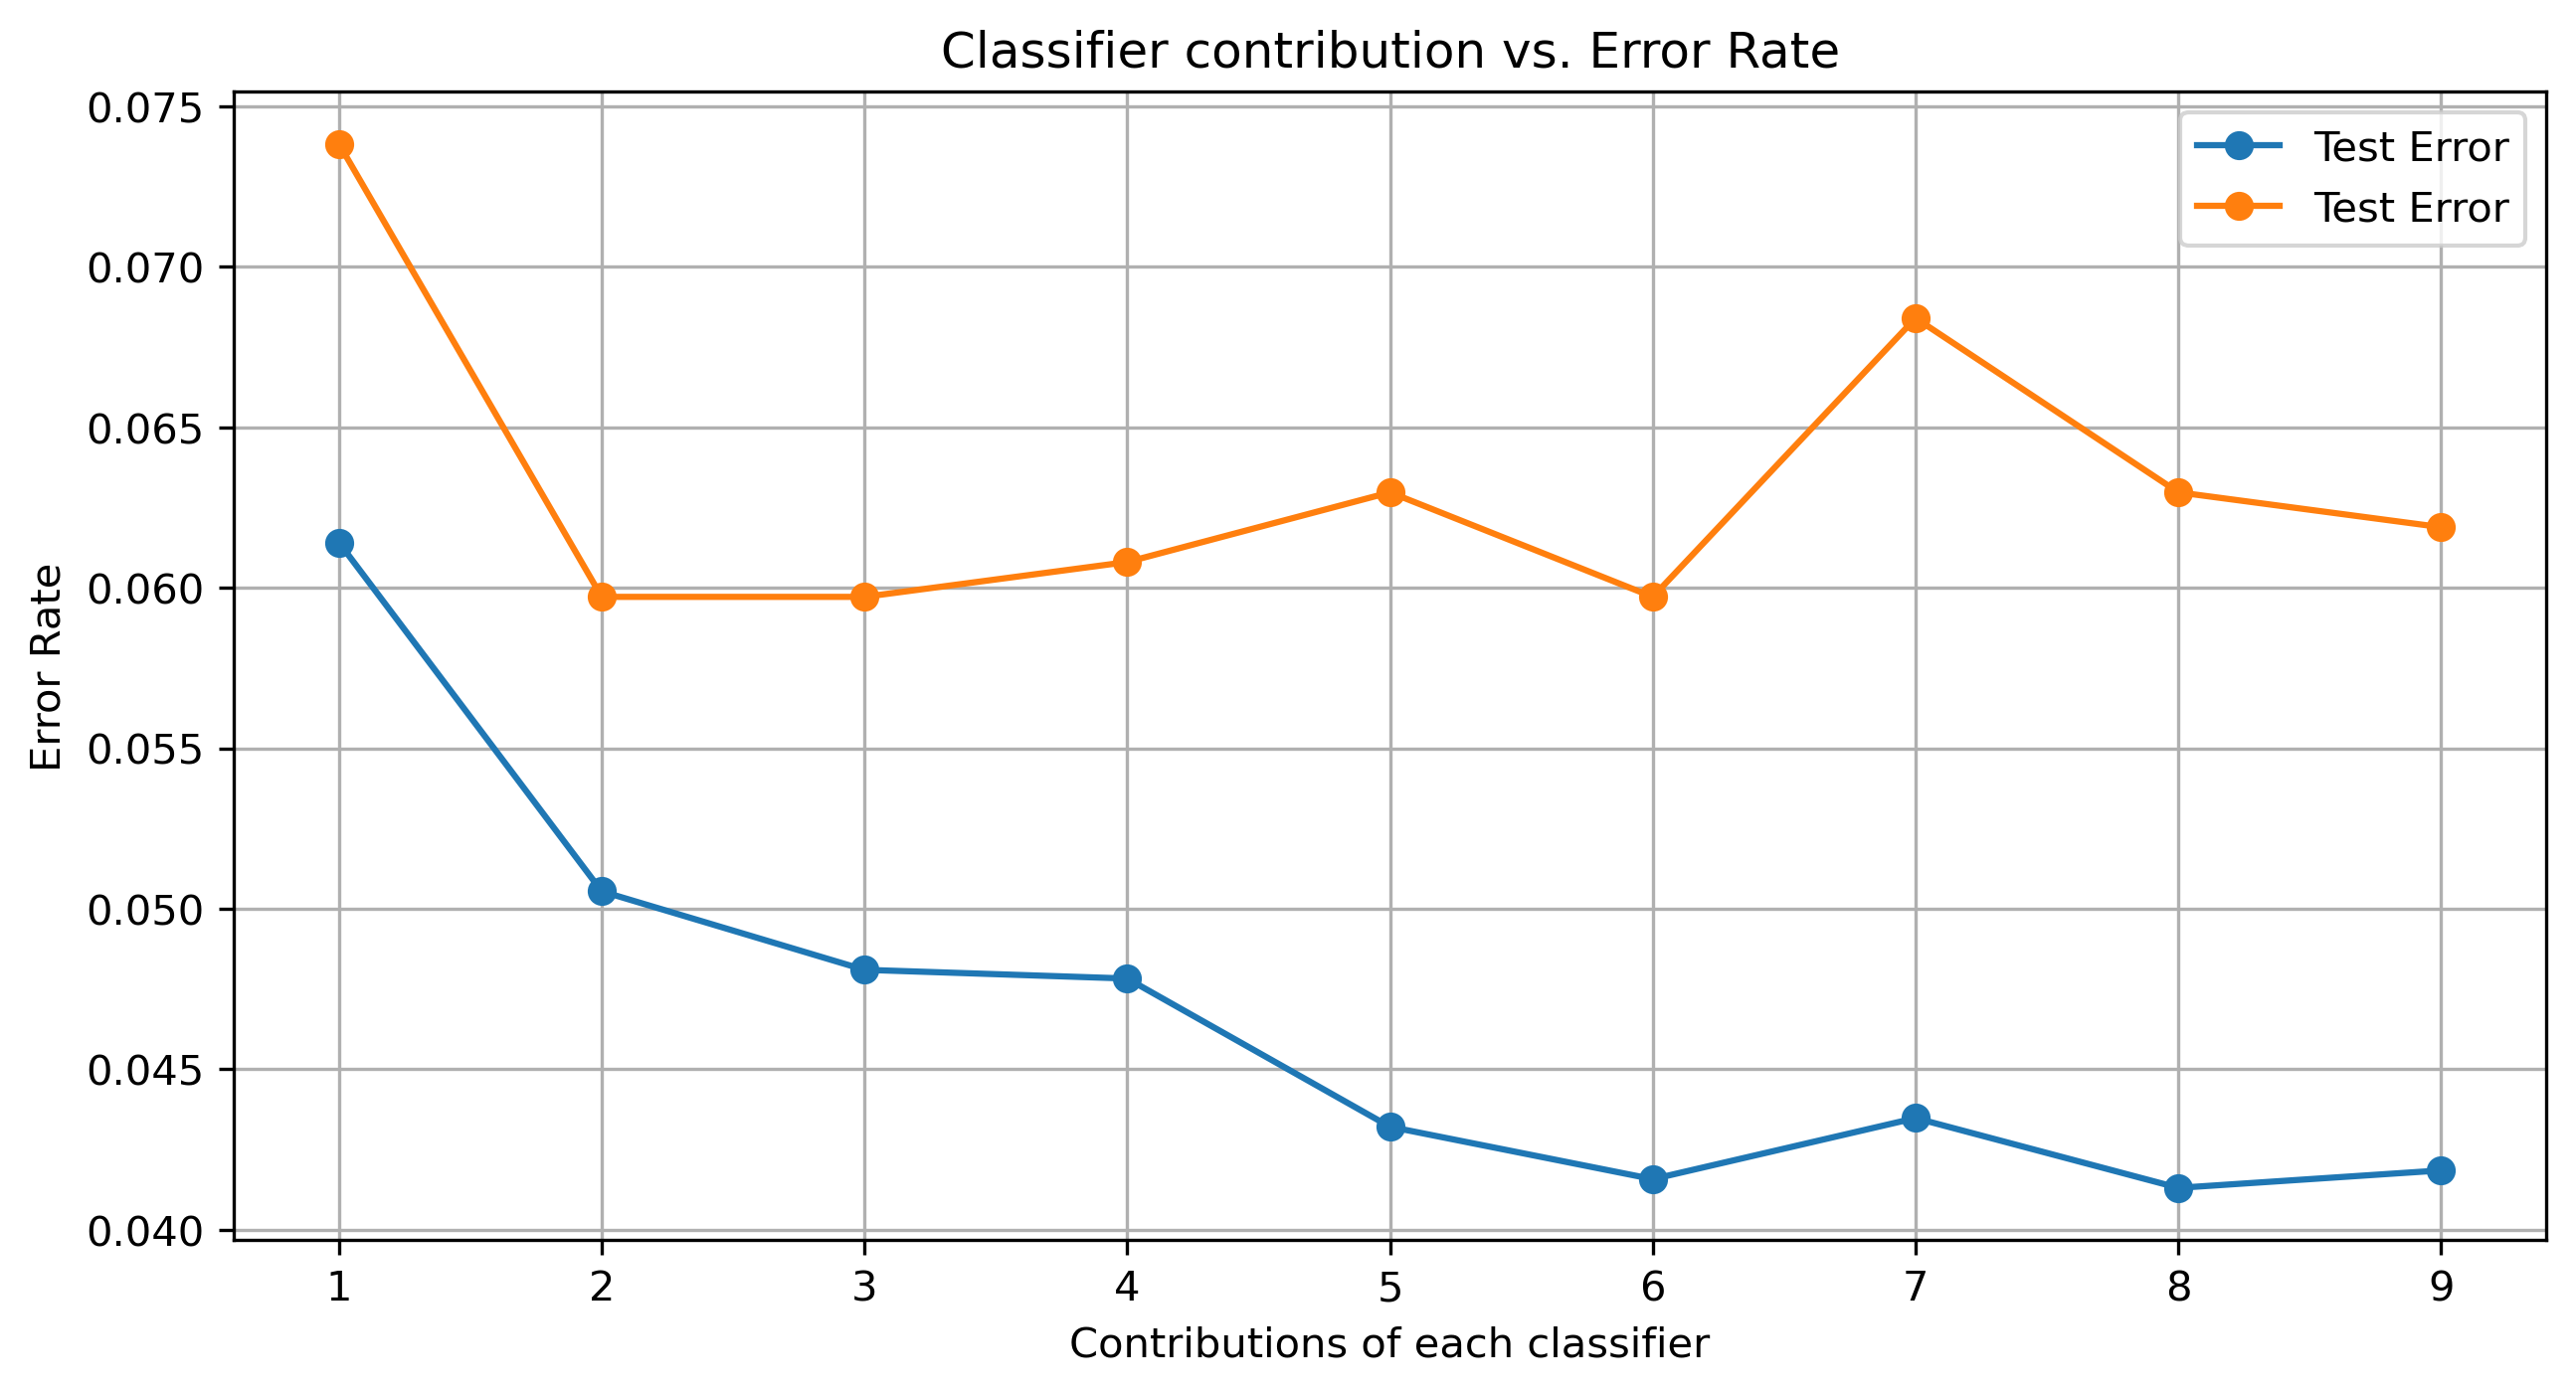
\includegraphics[width=0.8\linewidth]{figures/Boosted Trees/learn_rate_vs_error.png}
    \caption{Max stump size vs training and test error rate}
    \label{fig:boo}
\end{figure}

\begin{figure}[h!]
    \centering
    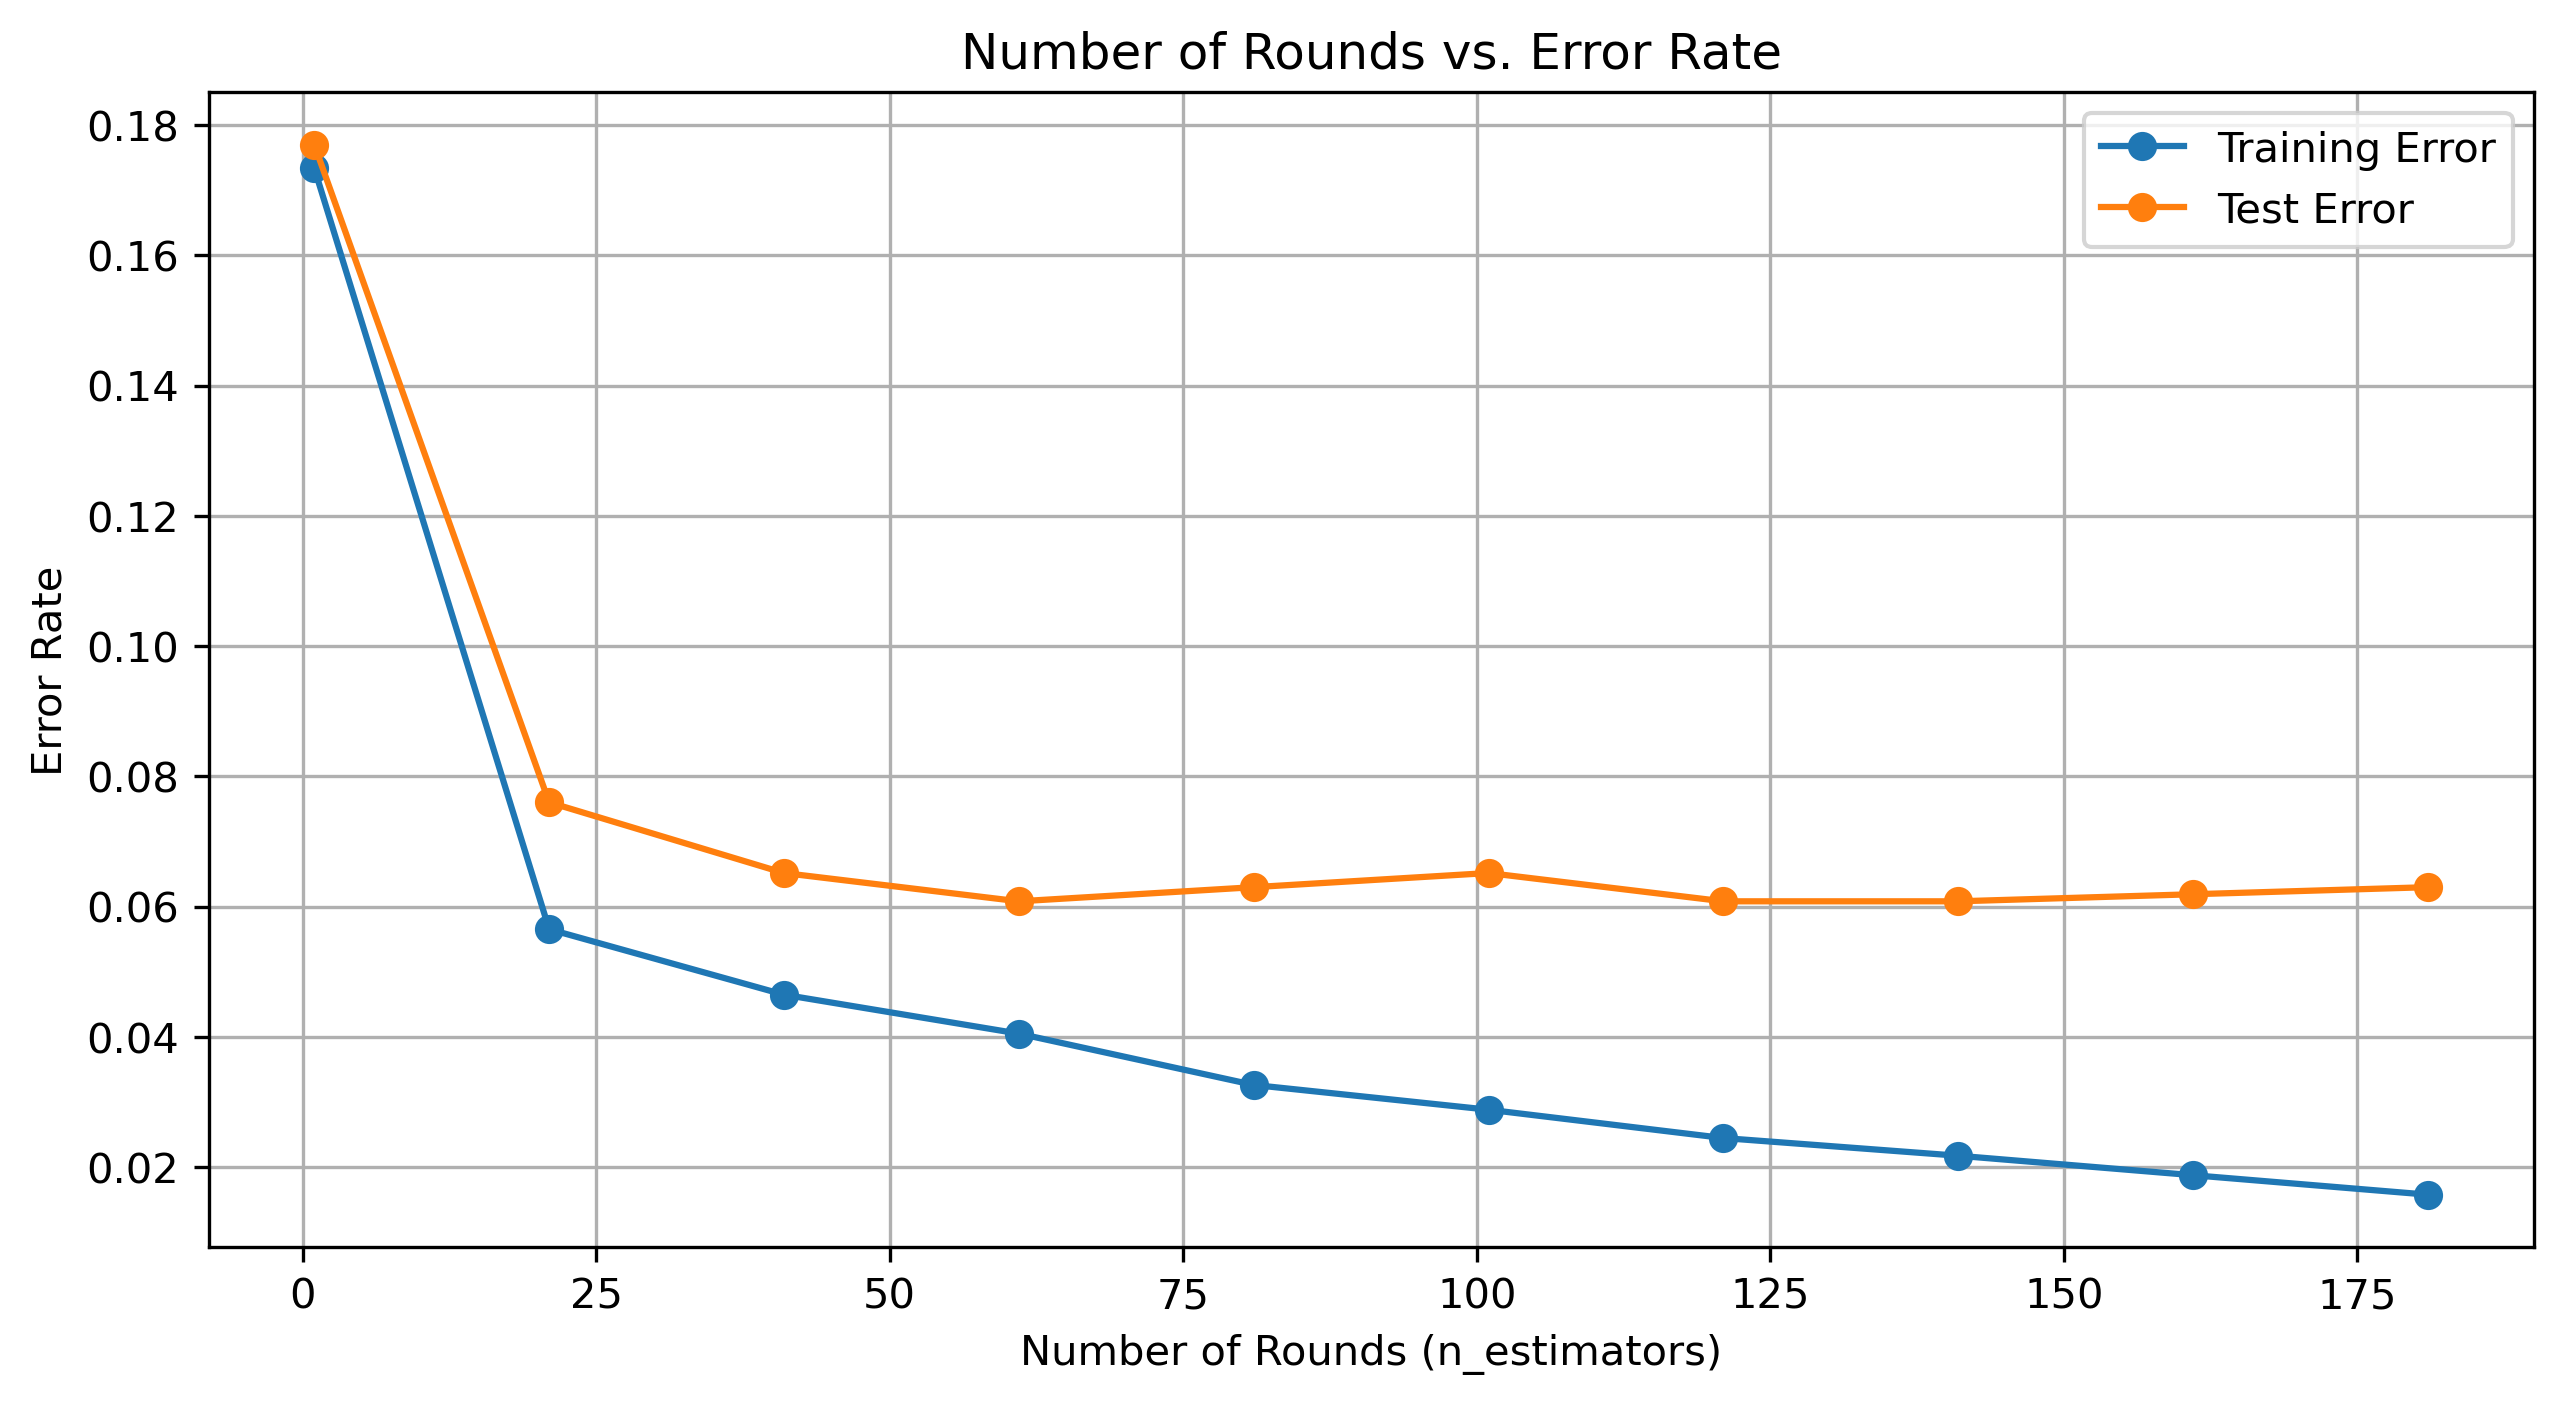
\includegraphics[width=0.8\linewidth]{figures/Boosted Trees/round_vs_error.png}
    \caption{Number of stumps vs training and test error rate}
    \label{fig:st}
\end{figure}
---

\section{Part II: Comparative Analysis}
This section compares the performance of random forests and boosted decision stumps. Key steps included:
\begin{itemize}
    \item Using k-fold cross-validation to tune the ensemble size for each method.
    \item Comparing test errors for the tuned versions of each method.
\end{itemize}
The graphs look the same. I'm pretty sure they're unique. Maybe. Probably.

\begin{figure}[h!]
    \centering
    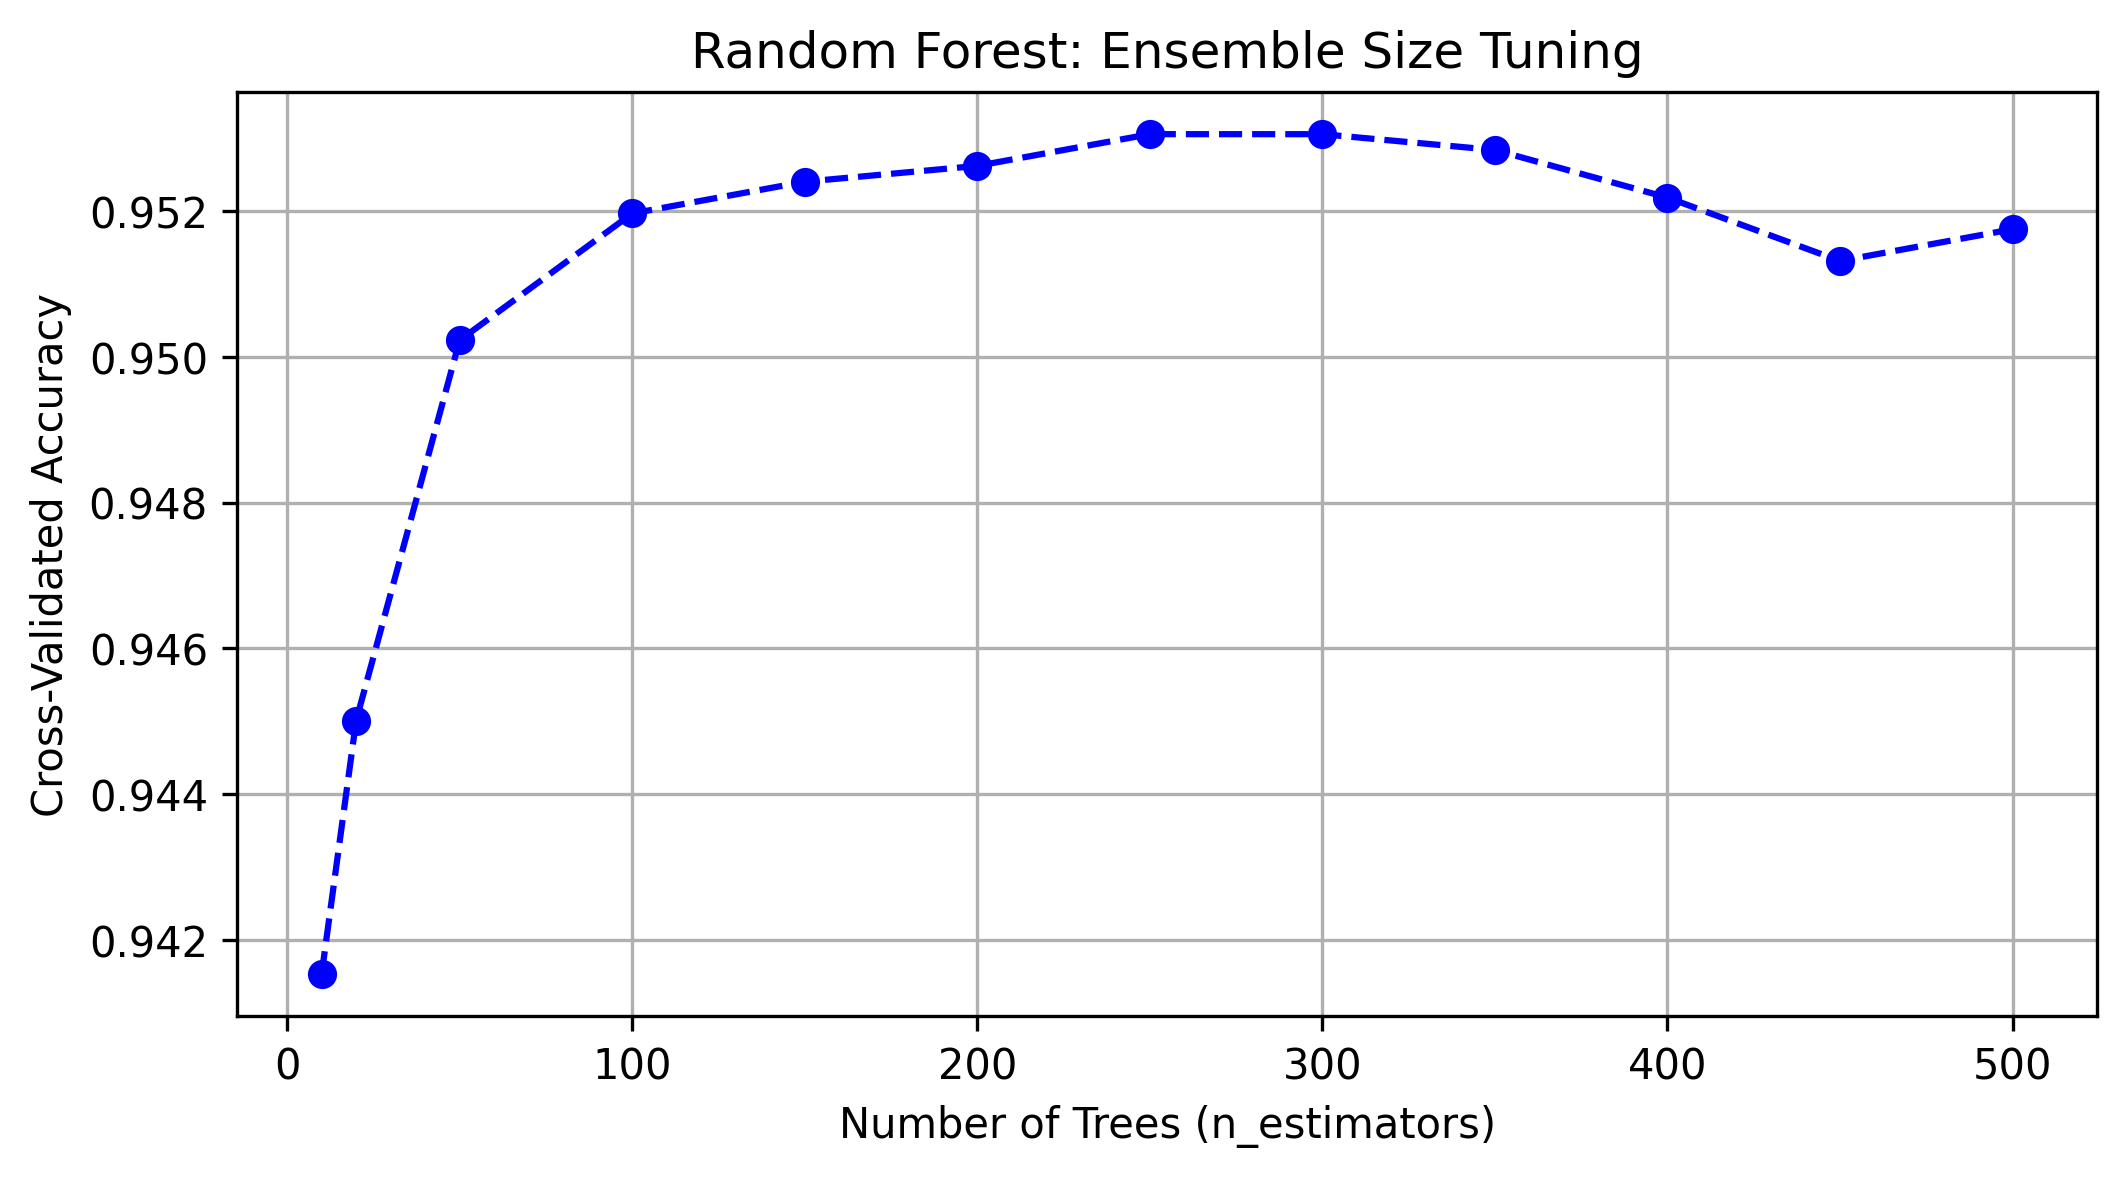
\includegraphics[width=0.8\linewidth]{figures/k-fold/ensemble_size_tuning.png}
    \caption{Random Forest Ensemble Size Tuning}
    \label{fig:kf}
\end{figure}

\begin{figure}[h!]
    \centering
    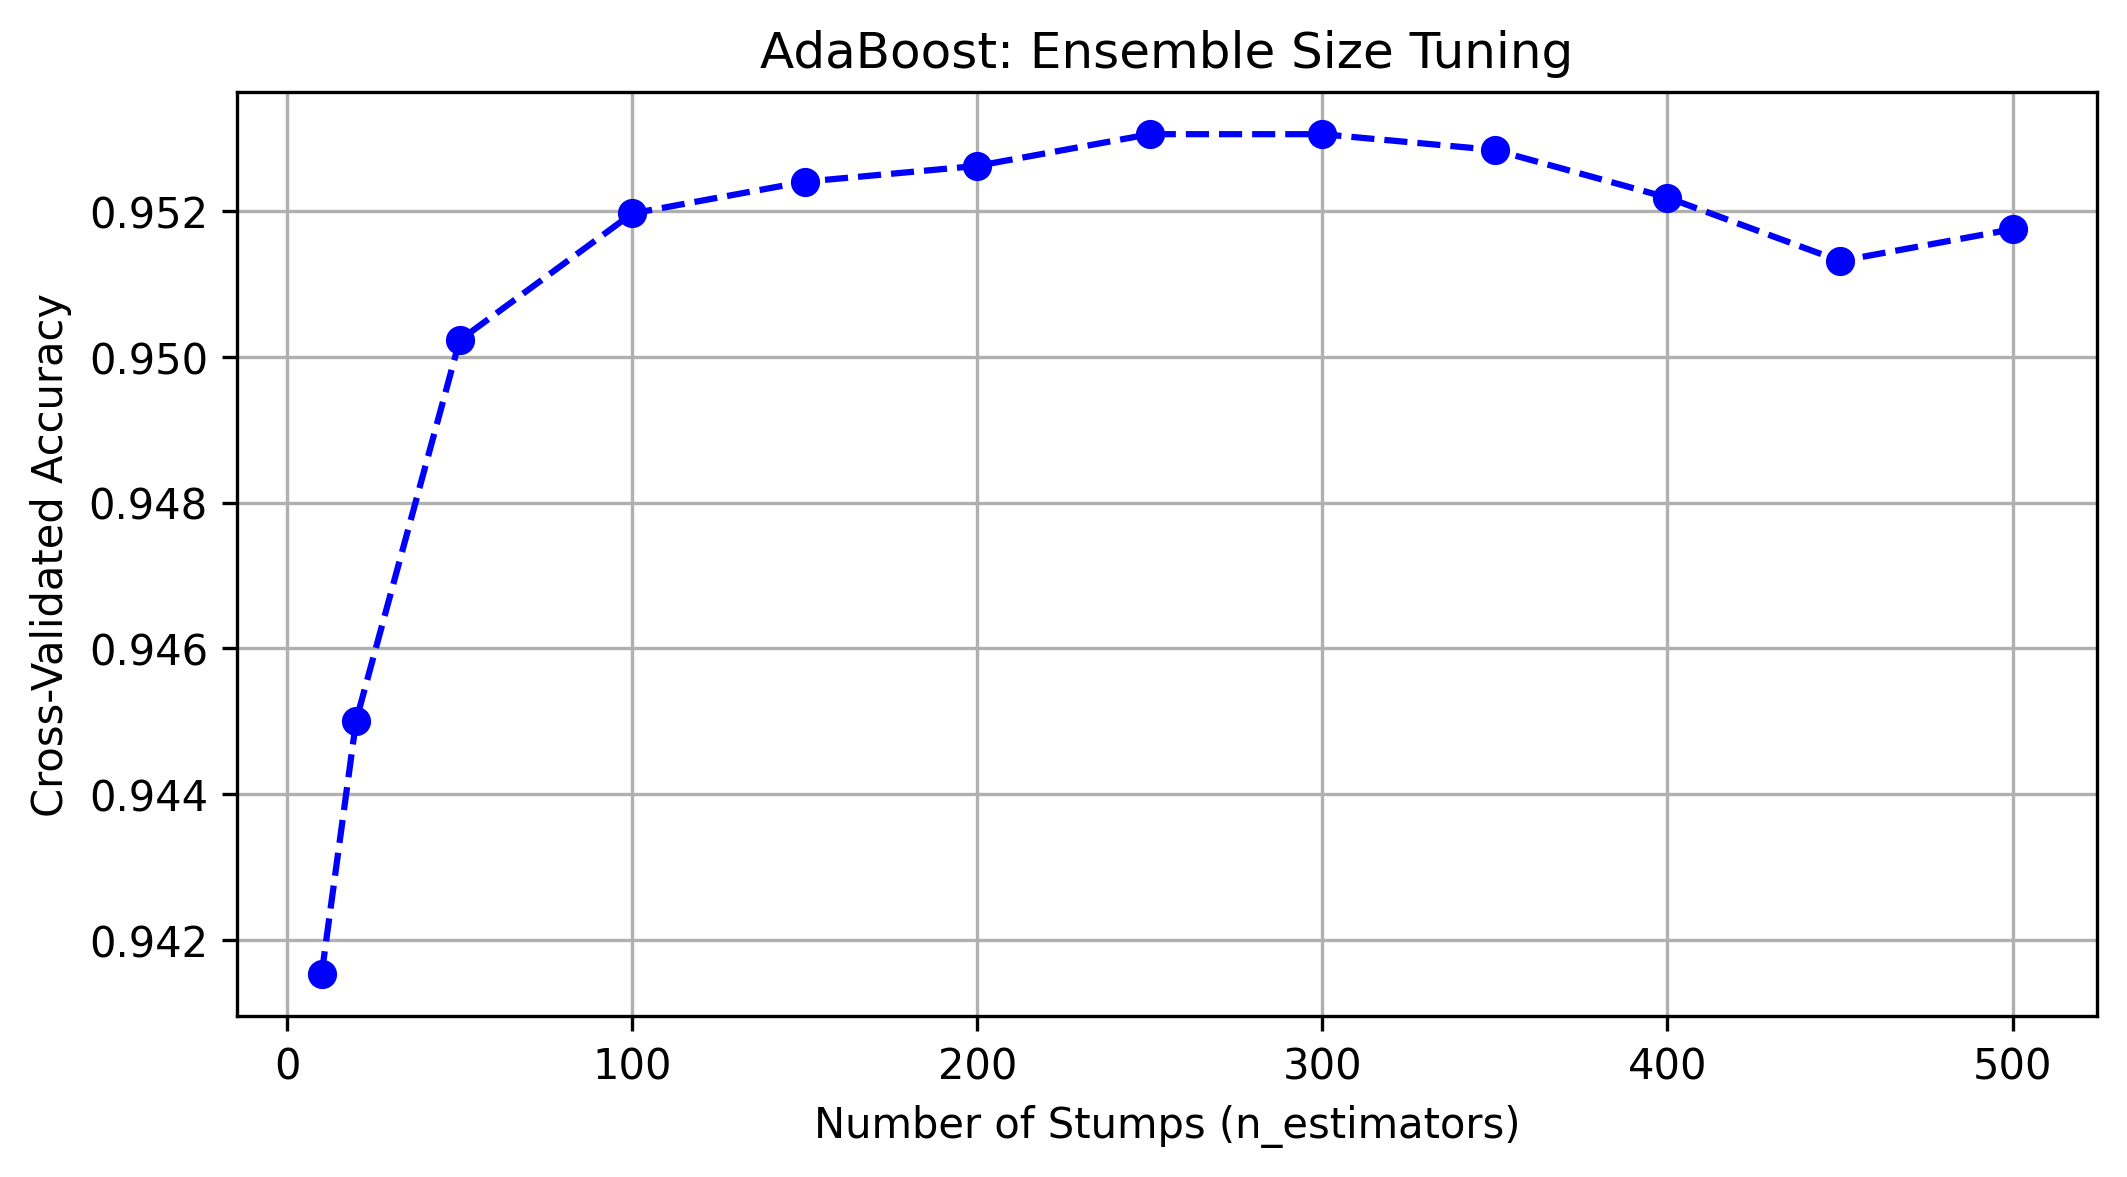
\includegraphics[width=0.8\linewidth]{figures/k-fold/ada_ensemble_size_tuning.png}
    \caption{AdaBoost Ensemble Size Tuning}
    \label{fig:old}
\end{figure}

---

\section{Out-of-Bag Error Estimate}
The out-of-bag (OOB) error estimate provides an unbiased measure of the generalization error for random forests. This section details the implementation and results of the OOB error analysis.

\subsection*{Implementation Details}
The OOB error was computed using a Random Forest classifier with \texttt{n\_estimators} ranging from 10 to 200. Hyperparameters such as \texttt{max\_depth} and \texttt{max\_features} were set to default values, and the OOB error was enabled via \texttt{oob\_score=True}. For each tree count, the OOB error was calculated as \( 1 - \text{oob\_score} \), where \texttt{oob\_score} represents the classification accuracy on out-of-bag samples.

\subsection*{Results}
Figure \ref{fig:oob_error} shows the OOB error as a function of the number of trees. The error stabilizes beyond approximately 100 trees, indicating that further increases in tree count yield minimal improvement.

\begin{figure}[h!]
    \centering
    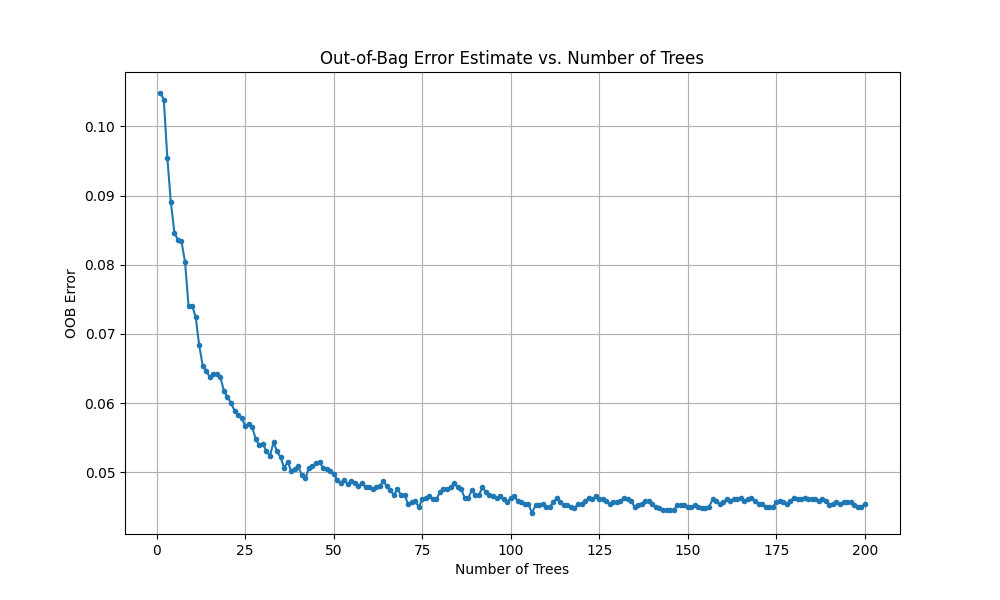
\includegraphics[width=0.8\linewidth]{figures/OOB_error.png}
    \caption{OOB Error vs. Number of Trees in the Random Forest. The error stabilizes as the number of trees increases, indicating convergence.}
    \label{fig:oob_error}
\end{figure}

\subsection*{Discussion}
The OOB error stabilizes at around 3\%, closely matching the test error. This confirms the utility of the OOB error as a reliable estimate of generalization performance without the need for a separate validation set.

---

\section{Conclusion}
This analysis evaluated the performance of decision trees, random forests, and boosted decision stumps on the Spambase dataset. Key findings include:
\begin{itemize}
    \item Pruning techniques significantly reduce overfitting in decision trees.
    \item Random forests achieve robust performance, with feature importance providing insights into the dataset.
    \item Boosted decision stumps, while computationally intensive, often yield higher accuracy.
\end{itemize}
Potential improvements include exploring additional hyperparameters and ensemble methods, as well as using larger datasets for more robust evaluation.

---

\section{References}
\begin{itemize}
    \item Spambase Dataset: \href{https://archive.ics.uci.edu/ml/datasets/Spambase}{UCI Machine Learning Repository}
    \item Scikit-learn Documentation: \href{https://scikit-learn.org/}{scikit-learn}
\end{itemize}
\end{document}